\documentclass[conference]{IEEEtran}
\usepackage{amsmath}
\usepackage{newtxtext,newtxmath}
\usepackage{graphicx}
\usepackage{booktabs}
\usepackage{tabularx}
\usepackage{array}
\usepackage{seqsplit}
\usepackage{fvextra}
\usepackage{url}
\usepackage[hidelinks]{hyperref}
\usepackage{microtype}
\setlength{\emergencystretch}{2em}
\DefineVerbatimEnvironment{Highlighting}{Verbatim}{breaklines,breakanywhere,fontsize=\small}
\newenvironment{Shaded}{}{}
\title{Arithmetic-Fair Comparisons of Exact FIR Software: A Cortex-M0 Model Case Study}
\author{\IEEEauthorblockN{Anonymous authors}}
\begin{document}
\pagestyle{plain}
\maketitle
\thispagestyle{plain}
\begin{abstract}

Arithmetic-range information can change an exact FIR implementation
decision. On a pinned Cortex-M0 model, replacing wide direct
accumulation by two certified int32 partial sums overturns two of four
original demand-Hcub transposition advantages. Hcub then costs
4.33\%/5.00\% more with GCC10 but 24.06\%/5.23\% less with GCC15, for
blocks 1/64. A prospectively frozen synthetic panel reproduces this
comparator boundary in 24 of 32 complete widening-required
fixed-compiler cells. Eight unavailable native-fit library identities
leave the full panel incomplete. Incremental sharing has a different
outcome: Hcub loses to ordinary transposition in all 32 fresh wide
cells, despite beating old direct/library controls. Exact saved-event
analysis separates arithmetic gains from RAM penalties; only original
GCC15/block1 retains Hcub's nominal advantages over both stronger
controls throughout an arbitrary RAM-weight stress over {[}0.5,2{]}. A
matched direct-kernel intervention exposes literal one-output knowledge,
removes reviewed next-output preparation and lowers GCC15 modeled cost
by 31.44\%. The direct compiler gap contracts from +70,469.699925 to
−11,857.443121 nJ, reversing that specialized pair's ranking. These
results support a bounded empirical case study of comparator fairness,
representation and compiler knowledge using established techniques.
Costs are configuration-specific event estimates; no new FIR algorithm,
general selector or physical-energy advantage is established.

\end{abstract}

\section{Introduction}\label{introduction}

Giving direct accumulation the same exact-range information as its
transposed competitor changes the implementation decision. For the
frozen nonsymmetric \texttt{speech\_minphase48} filter, demand-Hcub
transposition had lower modeled CPU energy than both wide specialized
direct and unrolled CMSIS in all four compiler/block cells. Retaining
the direct history layout but accumulating two certified native-width
partials overturns both GCC10 decisions; Hcub retains both GCC15 cells.
Arithmetic legality alone cannot predict that split.

Transposition exposes products of one sample with many constants,
enabling shared shift/add expressions. It also changes state meanings,
widths and lifetimes. We therefore distinguish three contrasts: partial
versus wide direct measures width correction within one organization;
Hcub versus ordinary transposition measures incremental sharing with
suffix equations fixed; and cross-compiler direct binaries, followed by
a single block-knowledge intervention, test a generated-code
explanation. Hcub versus corrected direct is the implementation choice,
combining sharing and representation.

The original strict four-cell reporting rule, \(H_R\), is retrospective
(Section 4.2). A separately frozen prospective panel asks whether
strengthening the nontransposed comparator overturns an old-control Hcub
advantage on fresh widening-required designs, across paired
amplitude/stream regimes. The matched direct intervention asks whether
exposing a one-output bound inside the callee removes identified
next-output preparation and reduces GCC15 cost and the compiler gap.

Range analysis, native partials, transposition, Hcub and specialization
are established techniques. Our contribution is finite empirical
evidence about which conclusions survive these controls, with exact
event sensitivity and portable raw evidence. Field priority and a
general implementation selector remain unestablished.

The fresh panel supplies wide-design reversal witnesses while rejecting
an extension of beneficial incremental sharing to those arrays. The
matched intervention removes the identified preparation, reduces GCC15
cost and reverses the direct compiler ranking. Together they sharpen the
original comparison into a boundary account, retaining negative and
unavailable outcomes.

\section{Closest prior work}\label{closest-prior-work}

De Coster et al.~{[}1{]} transform graphs for compiled bit-true DSP
simulation; their FIR example uses magnitude information to avoid
unnecessary overflow handling. Ménard and Sentieys {[}6{]} select
software word lengths/instructions under an SQNR constraint, including
arithmetic and transfer costs. Our full-int16 exact-output contract
differs from their accuracy constraint, but width selection and narrow
arithmetic are established techniques.

Gačić et al.~{[}2{]} generate FIR software with SPIRAL and show that
blocking and computation order alter runtime at equal arithmetic count.
D'Alberto et al.~{[}3{]} generate fixed-point XScale transforms and
optimize runtime and physically measured energy. FIR generation,
locality-aware search and energy-oriented selection therefore precede
this synthetic boundary comparison. Their physical measurements do not
validate our model costs.

Voronenko and Püschel's {[}4{]} Hcub shares arithmetic graphs across
constant products, with software concerns including register pressure
beyond addition count. Its objective is not an executable energy model.
Nikov et al.~{[}5{]} supply our configuration-specific event weights;
affine reweighting is elementary sensitivity analysis. GCC documents
constant propagation, cloning and interprocedural optimization {[}7{]};
fixed-bound specialization is conventional and those documents cannot
identify a historical responsible pass. Clean-copy artifact checks
likewise follow established practice {[}10{]}.

This targeted source challenge is not an exhaustive priority search.
Ménard--Sentieys §§4--5.4, SPIRAL FIR §§4--5, XScale and Nikov full
texts support the comparisons. Fresh Hcub full-text access supports
sharing (§1.2) and the register-pressure caveat (p.~6). De Coster
overlap uses fresh indexed primary excerpts plus recorded earlier
inspection; unsuccessful recent full-PDF retrieval licenses no exclusion
of unseen capabilities.

\section{Exact contract and controlled representations}\label{exact-contract-and-controlled-representations}

\subsection{Numeric semantics}\label{numeric-semantics}

All filters have 48 frozen signed-int16 coefficients, ordered so that
\(h[0]\) multiplies the newest sample. Every candidate must accept all
\(x\in[-32768,32767]\), including −32768, regardless of the amplitude
used for performance measurement. Initial history is zero. For requested
samples only,

\[
\begin{aligned}
S[n]&=\sum_{k=0}^{47}h[k]x[n-k],\\
Q(s)&=\min\{32767,\max\{-32768,\lfloor s/32768\rfloor\}\},\\
y[n]&=Q(S[n]),\qquad x[n]=0\text{ for }n<0.
\end{aligned}
\]

Exactly one final quantization and saturation is permitted. There is no
intermediate truncation, saturation or appended convolution tail. In
particular, \(Q(-1)=-1\); truncation toward zero at that boundary
changes the contract. The generated quantizer clamps before narrowing
and implements negative floor using C division without assuming
arithmetic signed right shift.

For each coefficient, exact independent-input product endpoints are
\(l_k=\min(-32768h_k,32767h_k)\) and \(u_k=\max(-32768h_k,32767h_k)\).
Summing those endpoints gives tight intervals for the full sum and any
specified group. A sign-aligned legal sample window attains each
endpoint. A sufficient group-prefix certificate also uses
\(32768\sum_{k\in G}|h_k|\le\mathrm{INT32\_MAX}\): every product and
accumulated prefix within \(G\) fits int32. Full intervals, prefix
bounds, transposed suffix bounds and Hcub primitive/restored-product
identities are separate certificates. C evaluation widths must respect
them; widening after an overflowing addition is too late.

\subsection{The original arithmetic correction}\label{the-original-arithmetic-correction}

The corrected original direct kernel keeps the same chronological
history and literal coefficient order. Fixed groups \([0,2)\) and
\([2,48)\) have coefficient L1 sums 12,778 and 59,731, hence absolute
prefix bounds 418,709,504 and 1,957,265,408. Both fit int32. The full L1
sum is 72,509, with absolute bound 2,375,974,912; legal sign-aligned
windows attain 2,375,922,255 and −2,375,955,060, establishing that
full-sum int32 overflow is possible. Each completed partial is converted
separately before the int64 reduction:

\begin{Verbatim}[breaklines,breakanywhere,breaksymbolleft={},breaksymbolright={},fontsize=\scriptsize]
int64_t exact_sum = (int64_t)partial0 + (int64_t)partial1;
y[j] = quant(exact_sum);
\end{Verbatim}

The split was fixed for the missing-control experiment. It is neither an
optimized partition nor a claim that the direct realization is optimal.

\begin{table*}[!t]
\centering\footnotesize
\caption{The five principal original forms; all satisfy the same final-output
contract.}\label{tab:1}
\begin{tabularx}{\textwidth}{@{}>{\raggedright\arraybackslash}X>{\raggedright\arraybackslash}X>{\raggedright\arraybackslash}X@{}}
\toprule
Short name & Original artifact identifier & Controlled role \\
\midrule
CMSIS & \texttt{cmsis64\_unroll} & Historical unrolled wide library control \\
Wide direct & \texttt{spec\_direct} & Specialized chronological direct, wide sum \\
Partial direct & \texttt{partial\_direct32x2} & Same direct history, two native partials \\
Ordinary transposed & \texttt{trans\_const} & Bounded suffix states, ordinary products \\
Hcub & \texttt{trans\_hcub\_demand} & Same suffix equations, shared constant products \\
\bottomrule
\end{tabularx}
\end{table*}

Ordinary transposition computes the current sum from \(h[0]x+z_0^{old}\)
and updates \(z_i\) from \(h[i+1]x+z_{i+1}^{old}\), ending with the last
product. Ascending updates preserve the required old states. Suffix
bounds justify each state's width. Hcub adds independently checked
shared expressions and demand-driven emission near their consuming
stage. Safe exact operations replace problematic signed shifts.

Figure 1 contrasts the value meanings and lifetimes. Direct state
retains input history; transposed state retains weighted suffix sums.
Correctness therefore reconstructs the intended values for each
representation instead of comparing unlike state bytes. Hcub versus
ordinary transposition holds those equations and layout fixed. Hcub
versus direct also changes representation; Hcub versus CMSIS changes
additional implementation choices. The entire library-relative saving
cannot be assigned to sharing.

\begin{figure*}[!t]
\centering
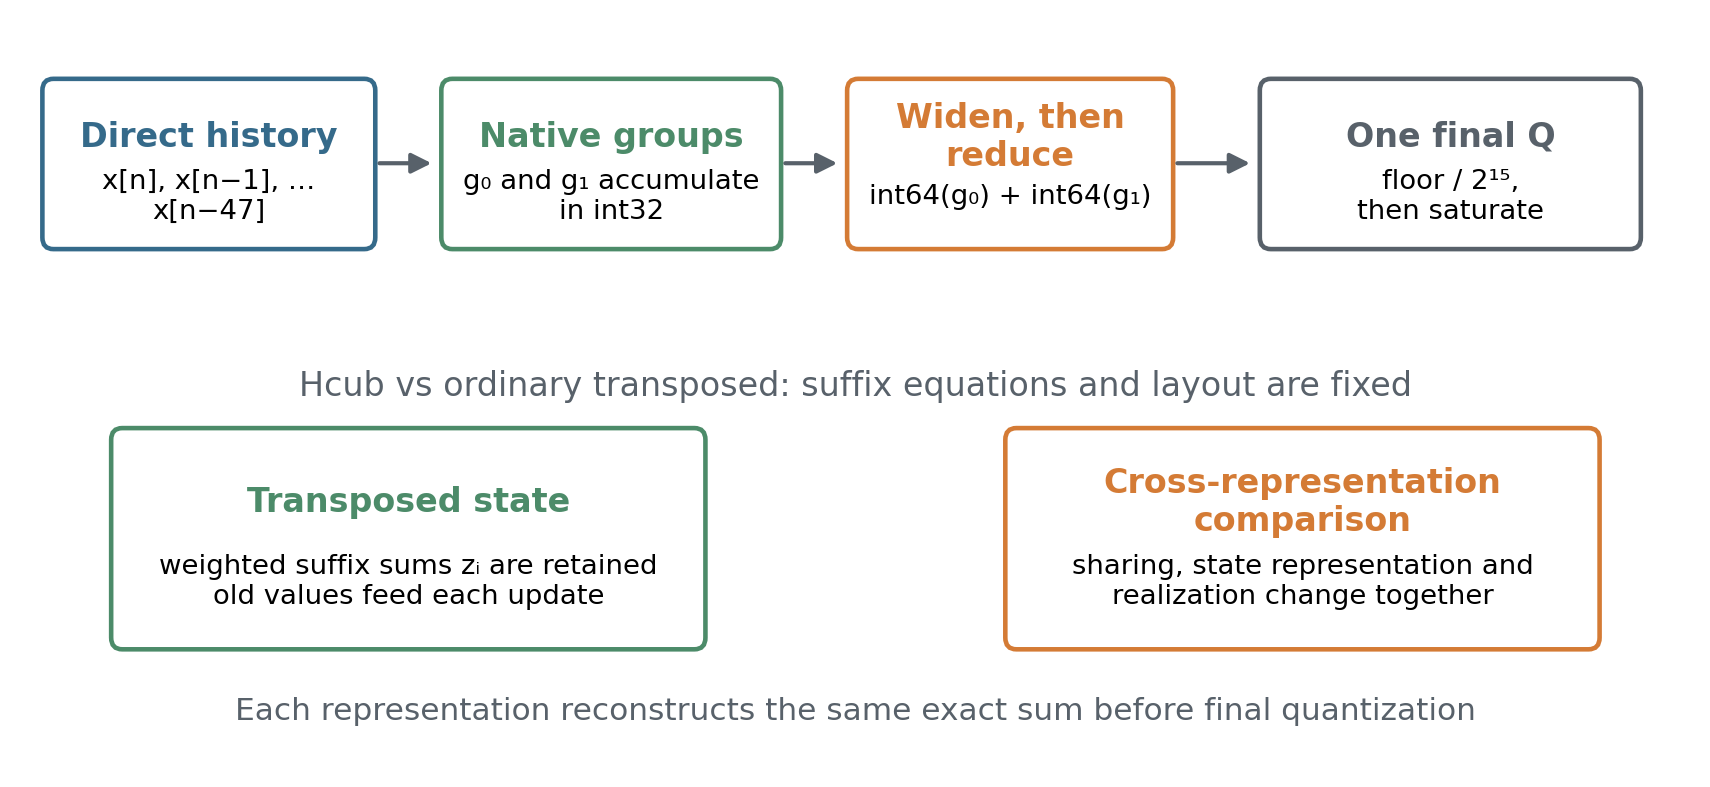
\includegraphics[width=\textwidth]{figures/representation-lifetime.png}
\caption{Exact representations and controlled contrasts. Each direct native group widens before reduction; both representations keep the exact sum until one final quantizer. Direct history and weighted suffix states have different meanings and lifetimes. The cross-representation comparison combines sharing and realization.}\label{fig:figures-representation-lifetime.png}
\end{figure*}

\section{Measurement, chronology and prospective questions}\label{measurement-chronology-and-prospective-questions}

\subsection{Target and event models}\label{target-and-event-models}

The target is Cortex-M0 Thumb at \texttt{-O2}, separate compilation and
no LTO. GCC10 reports 10.3.1 20210621; GCC15 is Arm GNU Toolchain
15.2.Rel1, reporting GCC 15.2.1 20251203. The simulator is pinned to
commit \texttt{\seqsplit{c55ea1b1926b792d7aabb7e3495b55a7b69ef134}}.
Code and coefficients reside in Flash, with state/input/output in SRAM.
Measurement includes dispatch, recurring calls, copies, convolution,
quantization, output stores and retained history/state movement,
including a final short call. Initialization, checking and printing lie
outside. The audited decoder removes the closing marker instruction
consistently.

Let \(N_I\) include all instructions, \(N_M\) native multiplication
instructions, \(B\) taken branches, \(R\) and \(W\) SRAM reads/writes,
\(F\) Flash data reads and \(N_{BL}\) branch-with-link instructions. The
zero-wait, single-cycle-MUL Arm-table cycle estimate is

\[T=N_I+R+W+F+2B+N_{BL}.\]

Nikov et al.'s {[}5{]} 20 MHz, prefetch-off, zero-wait weights give
modeled CPU energy in nJ:

\[
\begin{aligned}
E={}&0.964258(N_I-N_M)+1.652455N_M\\
 &+2.091986B+1.109833R+0.650563W+0.633621F.
\end{aligned}
\]

Their reported configuration MAPE is 2.80\%, an aggregate
model-validation statistic rather than an uncertainty bound for these
pairwise margins. The fitted weights may absorb correlation/residual
effects; they are not independently measured physical event prices. We
retain integer events and exact six-decimal products. The 0.000001 nJ
tolerance for historical floating serialization is solely a
data-admission tolerance.

\subsection{Admission and evidence chronology}\label{admission-and-evidence-chronology}

The original pre-evaluation protocol covered three designs, two input
guarantees, two blocks and two compilers. A source-level state-traffic
estimate was later withdrawn as an optimistic floor: grouped
transfers/register retention could reduce it, and no candidate had been
excluded using it. Observed unequal width treatment then motivated the
fixed two-group/four-cell correction, followed by the compiler account.
\(H_R\) was formulated afterward, so it is retrospective. Previously
inspected filters remain development evidence; the fresh panel and
intervention were frozen before target costs.

For the original 257-sample zero-history saved \texttt{adc\_raw} stream,
block1 makes 257 calls; block64 makes four full calls and one one-sample
call. The reporting rule is \(r=100(E_H/E_P-1)\) with Hcub \(H\) and
partial direct \(P\). \(H_R\) survives only if all four admitted values
are strictly negative. A tie fails strict superiority;
missing/inadmissible evidence makes assessment unavailable. This is a
deterministic criterion, without sampling variance or significance
testing.

Arithmetic certificates establish full-domain source legality; finite
UBSan, target output/state/guard checks address implementation errors.
The original independent check admitted 1,028 new, 6,168 historical and
722 signed-edge output comparisons. Emitted-code review confirmed native
partials/wide final reduction in all four corrected binaries.
Source/binary hashes bind events to checked code. Pinned library
semantics, including fast-CMSIS eligibility, require source/toolchain
admission beyond finite agreement.

\subsection{Saved-event analysis}\label{saved-event-analysis}

For each compiler/block we analyze exactly three oriented pairs: partial
minus wide direct, Hcub minus ordinary transposition and Hcub minus
partial direct. All use the same 257 outputs. With
\(v=(N_I-N_M,N_M,B,R,W,F)\) and the weights above,
\(\Delta E=w\cdot\Delta v\); negative favors the left form. Six-event
dominance requires all coordinates nonpositive with at least one
strictly negative; mixed signs preclude it. Resources are excluded.

One predeclared arbitrary stress multiplies both RAM weights by
\(\lambda\), leaving the other four fixed. For \(\lambda\ge0\),

\[
\begin{aligned}
\Delta E(\lambda)&=A+B_{RAM}\lambda,\\
B_{RAM}&=1.109833\Delta R+0.650563\Delta W.
\end{aligned}
\]

The selected closed region is \([0.5,2]\). It is an uncalibrated
coefficient stress, not a confidence interval, hardware configuration or
physical-price range. Integer-weight products retain exact decimal
values; boundaries are exact rational \(-A/B_{RAM}\) values. Rounded
roots are display only. Endpoint signs decide strict ordering throughout
the region by linearity; any tie defeats strictness. The artifact
retains all 12 vectors, cost components, resource deltas and root
classifications, including negative algebraic roots.

\subsection{Frozen synthetic panel}\label{frozen-synthetic-panel}

Three fresh nonsymmetric gain-normalized 48-tap designs deliberately
span one native-sum and two widening-required regimes. With NumPy
1.26.4/SciPy 1.15.3, we apply
\texttt{firwin(95,\ cutoff,\ fs=16000,\ window=window,\ scale=True)},
homomorphic \texttt{minimum\_phase(half=True,n\_fft=32768)}, target-L1
scaling and \texttt{np.rint} integer rounding. The half-length
conversion changes prototype magnitude {[}8{]}. These are synthetic
arithmetic controls, not representative application filters.

\begin{table*}[!t]
\centering\footnotesize
\caption{Frozen arithmetic regimes, independently prepared before target costs.
Cuts give first-legal / range-balanced two-group boundaries.}\label{tab:2}
\begin{tabularx}{\textwidth}{@{}>{\raggedright\arraybackslash}X>{\raggedright\arraybackslash}X>{\raggedright\arraybackslash}X>{\raggedright\arraybackslash}X>{\raggedright\arraybackslash}X@{}}
\toprule
Design & Cutoff/window & Target / actual L1 & Exact full-sum interval & Direct cuts \\
\midrule
\texttt{native\_lp1800} & 1800 Hz / Hamming & 50000 / 50001 & {[}−1638421124,1638394411{]} & Whole native sum \\
\texttt{wide\_lp2800} & 2800 Hz / Hamming & 100000 / 100002 & {[}−3276839180,3276791890{]} & 4 / 5 \\
\texttt{wide\_lp4600} & 4600 Hz / Blackman & 110000 / 110003 & {[}−3604545833,3604500772{]} & 3 / 4 \\
\bottomrule
\end{tabularx}
\end{table*}

The first cut is the smallest legal two-group boundary; the balanced cut
minimizes the larger group L1, breaking ties by smaller boundary.
Sign-aligned legal windows attain both full-sum endpoints, proving
actual int32 overflow possibility in wide designs. Arrays, certificates,
graphs, stimuli and case list were frozen by hash before costs; no
outcome-driven replacement occurs.

Each design has six forms: wide direct, first certified direct, ordinary
transposed, demand-Hcub and standard unrolled CMSIS, plus native-only
fast CMSIS or wide-only balanced direct. All receive identical
coefficients, full-int16 semantics, block knowledge and generation
budget. Pinned CMSIS-DSP v1.14.4 paths receive reversed
coefficients/required storage, with separate source/compiler eligibility
and no fast-path scaling {[}9{]}. Each Hcub graph uses one unchanged
\texttt{acm\ -b\ 15\ -seed\ 1\ -nofs\ -gc} run on sorted odd
fundamentals.

The frozen 1089-sample full-range LCG master and samplewise
\texttt{full//32} ADC partner are specified in the linked protocol.
Startup measures its first 257 outputs from zero history. Post-startup
processes 64 samples outside the region, then measures offsets
{[}64,1089), retaining history: 1025 outputs. Both block sizes align at
the warm boundary; block64 ends with one short call in each regime.
Checks cover the entire prefix, including warmup. The region contrast
also changes segment and length, so it does not isolate startup cost.

The cap is 288 performance identities (3 designs × 6 forms × 2 compilers
× 2 blocks × 2 amplitudes × 2 regimes). Separate correctness admission
uses at most 72 target identities on the frozen 194-sample
zero/extremal/edge stream and host UBSan mixed partitions. Actual
image/call-chain bounds must fit the original 64 KiB Flash/8 KiB RAM
limits. Unsupported and failed cases remain visible; deterministic
executions are not independent statistical samples.

For each fixed-compiler cell, define \(D_{old}\) as the minimum eligible
old nontransposed control (wide direct, standard CMSIS, and fast CMSIS
where eligible). \(D_{new}\) is the minimum after adding both available
certified direct forms. All ties retain every minimizer. The primary
extension requires at least one admitted cell of either
widening-required design with \(E_H<D_{old}\) but \(E_H\ge D_{new}\). If
no such cell exists among the complete wide-required cells, the
extension is refuted; an unavailable required cell leaves the full-panel
assessment incomplete. Additional reports retain all-form winners, each
certified/wide percentage, Hcub/ordinary percentages, events/resources
and all amplitude/regime contrasts. Compiler-selectable decisions
minimize each form across compilers first, separately from
fixed-compiler results. Reference sums also count the two quantizer
clamp conditions, \(S\ge1073741824\) and \(S\le-1073741824\), in each
measured region. Output endpoints alone cannot identify those paths.

\subsection{Matched block-knowledge intervention}\label{matched-block-knowledge-intervention}

The intervention fixes the original block1 fixture and 257-sample
stream, with two compilers × general/specialized kernels. General kernel
bytes, wrapper, ABI and flags remain original. Only expression uses of
runtime \texttt{b} inside specialized \texttt{probe\_process} become
literal \texttt{1}, adding \texttt{(void)b;}. Every call meets \(b=1\);
arithmetic, groups, quantizer, state/history algorithm and separate
compilation/no LTO stay fixed. Four signed-edge target checks and
repeated-one-sample host checks support correctness. Failure to
reproduce general-control binary bytes/events stops historical causal
interpretation.

Define \(G_g=E_{15,general}-E_{10,general}\) and
\(G_s=E_{15,specialized}-E_{10,specialized}\), with saved
\(G_g=70469.699925\) nJ. The stronger outcome requires preparation
removal in reviewed emitted code, lower GCC15 cost and \(G_s<G_g\). Full
event/cycle and separate resource deltas test each condition. All total
changes belong to block-knowledge specialization; transfer-subset
attribution needs additional accounting. The direct-only intervention
licenses no other-form ranking or compiler-pass claim.

\section{Admitted original comparison and exact saved-event results}\label{admitted-original-comparison-and-exact-saved-event-results}

\subsection{Width correction changes two decisions}\label{width-correction-changes-two-decisions}

The stronger direct control lowers modeled CPU energy in all four cells,
by 32.823801\%, 41.860155\%, 23.440506\% and 41.980694\% relative to
wide direct, in GCC10/1, GCC10/64, GCC15/1, GCC15/64 order. It weakly
improves every one of the six event coordinates in each cell, with
strict improvements: the correction is six-event-dominant within this
saved comparison. This does not establish physical or resource
dominance. All five forms' complete costs remain visible below.

\begin{table*}[!t]
\centering\footnotesize
\caption{Original modeled CPU energy, nJ/requested output; all process the same
257 samples. Display rounding does not determine winners.}\label{tab:3}
\begin{tabularx}{\textwidth}{@{}>{\raggedright\arraybackslash}X>{\raggedright\arraybackslash}X>{\raggedright\arraybackslash}X>{\raggedright\arraybackslash}X>{\raggedright\arraybackslash}X@{}}
\toprule
Variant & GCC10 b1 & GCC10 b64 & GCC15 b1 & GCC15 b64 \\
\midrule
CMSIS & 1537.21 & 905.94 & 1503.18 & 838.85 \\
Wide direct & 1543.04 & 990.40 & 1712.07 & 1023.10 \\
Partial direct & \textbf{1036.55} & \textbf{575.81} & 1310.75 & 593.59 \\
Ordinary transposed & 1045.78 & 605.66 & 1039.99 & 602.87 \\
Hcub & 1081.44 & 604.62 & \textbf{995.43} & \textbf{562.55} \\
\bottomrule
\end{tabularx}
\end{table*}

\begin{table*}[!t]
\centering\footnotesize
\caption{\(100(E_H/E_{named}-1)\). Both historical comparisons favor Hcub in all
four cells. The corrected comparison rejects \(H_R\) with two surviving
cells.}\label{tab:4}
\begin{tabularx}{\textwidth}{@{}>{\raggedright\arraybackslash}X>{\raggedright\arraybackslash}X>{\raggedright\arraybackslash}X>{\raggedright\arraybackslash}X@{}}
\toprule
Compiler/block & Hcub / wide direct & Hcub / CMSIS & Hcub / partial direct \\
\midrule
GCC10/1 & −29.91\% & −29.65\% & +4.330785\% \\
GCC10/64 & −38.95\% & −33.26\% & +5.002907\% \\
GCC15/1 & −41.86\% & −33.78\% & −24.056759\% \\
GCC15/64 & −45.01\% & −32.94\% & −5.229188\% \\
\bottomrule
\end{tabularx}
\end{table*}

For GCC10/block64, partial direct executes 129,481 instructions and
2,827 MULs; Hcub executes only 116,139 instructions and 257 MULs. Yet
Hcub incurs 10,994 additional RAM reads and 18,235 additional writes.
Its complete modeled cost is 604.62 versus 575.81 nJ/output. Graph nodes
therefore do not determine the implementation winner.

Fixed versus selectable compiler decisions also differ. With GCC15
fixed, Hcub is 24.06\% and 5.23\% below partial direct. If either
compiler may be chosen separately for each form, GCC15 supplies the best
tested Hcub and GCC10 the best partial direct; the savings become 3.97\%
and 2.30\%. These minima cover only the tested builds and are not
calibrated physical-energy margins.

\subsection{Incremental sharing is smaller and event-mixed}\label{incremental-sharing-is-smaller-and-event-mixed}

Within the same transposed equations, Hcub costs more at GCC10/block1
and less in the other three nominal cells. Every incremental-sharing
event vector is mixed: fewer native MULs and Flash reads coexist with
additional RAM transfers. GCC10/block1 has no non-MUL instruction
reduction at all.

\begin{table*}[!t]
\centering\footnotesize
\caption{Hcub minus ordinary transposition, whole 257-output stream; percentage
denominator is ordinary transposition. Vector coordinates are
\((\Delta nonMUL,\Delta MUL,\Delta B,\Delta R,\Delta W,\Delta F)\);
nonMUL is \(N_I-N_M\).}\label{tab:5}
\begin{tabularx}{\textwidth}{@{}>{\raggedright\arraybackslash}X>{\raggedright\arraybackslash}X>{\raggedright\arraybackslash}X>{\raggedright\arraybackslash}X@{}}
\toprule
Compiler/block & \(\Delta v\) & \(\Delta E\), nJ & Relative \\
\midrule
GCC10/1 & (0, −2570, 0, 9509, 5397, −1028) & +9166.318770 & +3.410536\% \\
GCC10/64 & (−9324, −2570, 0, 9257, 5145, −1028) & −268.042614 & −0.172202\% \\
GCC15/1 & (−17990, −2570, −257, 7196, 5140, −1028) & −11452.561472 & −4.284890\% \\
GCC15/64 & (−17234, −2570, −5, 7196, 4888, −1028) & −10360.343828 & −6.686823\% \\
\bottomrule
\end{tabularx}
\end{table*}

For GCC15/block64, the 32.94\% Hcub/CMSIS saving becomes 6.686823\%
against ordinary transposition and 5.229188\% against corrected direct.
Only the first of those stronger contrasts holds suffix equations fixed.

Resource deltas are separate from event dominance. Hcub and ordinary
transposition allocate equal state; Hcub's reported process frame is 72
bytes larger in every cell, while selected kernel/coefficient symbols
are 36 bytes smaller with GCC10 and 180 with GCC15. Partial and wide
direct allocate equal state; partial direct has reported frames smaller
by 368, 368, 368 and 376 bytes and selected symbols smaller by 700, 524,
500 and 572 bytes. State allocation, compiler process frame and
selected-symbol bytes measure different things and are not added as
memory use. Appendix A retains every original principal row.

\subsection{Nominal winners under the arbitrary RAM-weight stress}\label{nominal-winners-under-the-arbitrary-ram-weight-stress}

The exact affine analysis reconciles all 12 nominal differences with the
admitted original energy totals. Partial minus wide direct has \(A<0\)
and \(B_{RAM}<0\) in every cell, so its six-event result also yields
lower modeled cost throughout the selected region and indeed for every
\(\lambda\ge0\). All eight Hcub contrasts are mixed, with \(A<0\) and
\(B_{RAM}>0\): their non-RAM benefit is eventually outweighed along this
chosen stress path.

\begin{table*}[!t]
\centering\footnotesize
\caption{Exact coefficients, rounded roots; cell abbreviates compiler/block. The
four negative roots lie outside the permitted \(\lambda\ge0\) domain.
Exact rational roots and endpoint winners are in the machine-readable
analysis.}\label{tab:6}
\begin{tabularx}{\textwidth}{@{}>{\raggedright\arraybackslash}X>{\raggedright\arraybackslash}X>{\raggedright\arraybackslash}X>{\raggedright\arraybackslash}X>{\raggedright\arraybackslash}X>{\raggedright\arraybackslash}X@{}}
\toprule
Pair (left − right) & Cell & \(A\), nJ & \(B_{RAM}\), nJ & Root (display) & Strict lower on {[}0.5,2{]}? \\
\midrule
Partial − wide & 10/1 & −87520.461808 & −42645.678958 & −2.052270 & Yes \\
Partial − wide & 10/64 & −64652.689002 & −41894.635425 & −1.543221 & Yes \\
Partial − wide & 15/1 & −62253.689535 & −40885.154171 & −1.522648 & Yes \\
Partial − wide & 15/64 & −69714.748911 & −40667.649816 & −1.714256 & Yes \\
Hcub − ordinary & 10/1 & −4898.171738 & 14064.490508 & 0.348265 & No; higher throughout \\
Hcub − ordinary & 10/64 & −13888.913330 & 13620.870716 & 1.019679 & No; changes sign \\
Hcub − ordinary & 15/1 & −22782.813560 & 11330.252088 & 2.010795 & Yes \\
Hcub − ordinary & 15/64 & −21526.654040 & 11166.310212 & 1.927822 & No; changes sign \\
Hcub − partial & 10/1 & −32436.319000 & 43973.275423 & 0.737637 & No; changes sign \\
Hcub − partial & 10/64 & −16661.004146 & 24064.520307 & 0.692347 & No; changes sign \\
Hcub − partial & 15/1 & −94335.682384 & 13297.172804 & 7.094417 & Yes \\
Hcub − partial & 15/64 & −16351.634074 & 8374.315001 & 1.952594 & No; changes sign \\
\bottomrule
\end{tabularx}
\end{table*}

Figure 2 shows why only GCC15/block1 stays below both controls
throughout {[}0.5,2{]}. GCC10/block64's incremental benefit changes sign
near 1.019679; GCC15/block64 crosses against both controls before 2.
GCC10's Hcub/partial losses reverse below their respective roots within
the region. These fixed-event boundaries neither identify real RAM
prices nor establish physical robustness.

\begin{figure*}[!t]
\centering
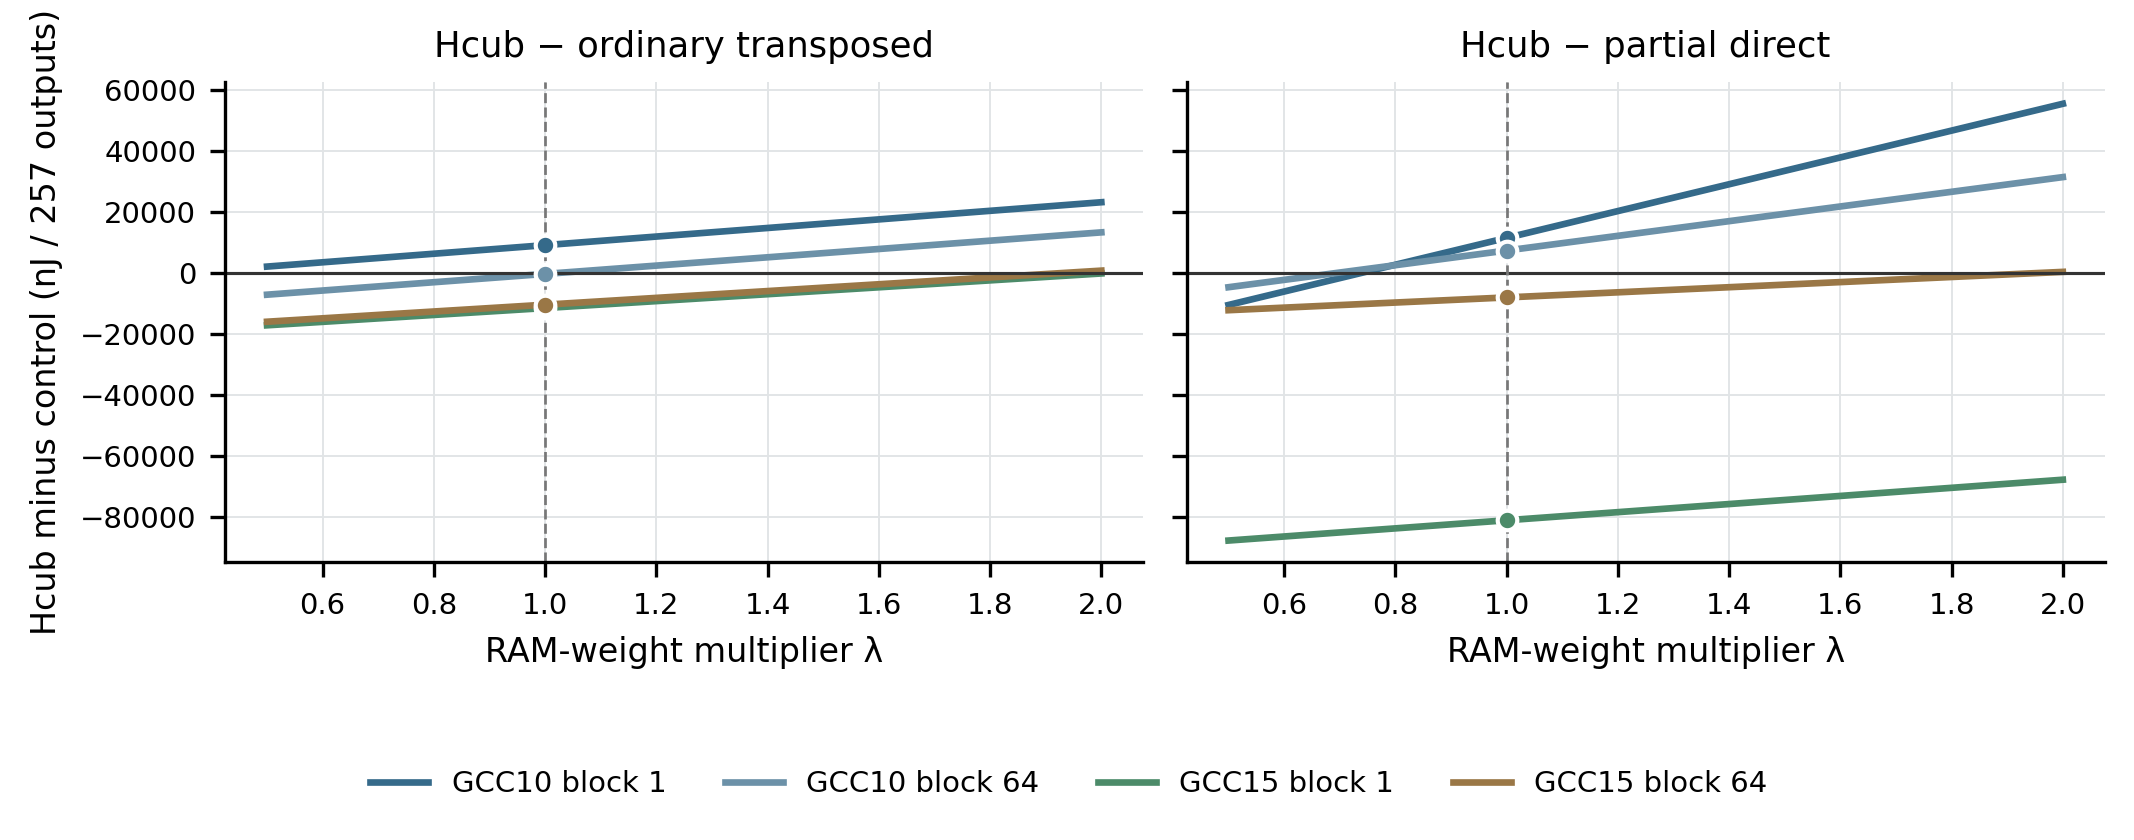
\includegraphics[width=\textwidth]{figures/ram-sensitivity.png}
\caption{Saved-event RAM-weight sensitivity for Hcub minus ordinary transposition and Hcub minus corrected direct. Negative differences favor Hcub. Lines reuse fixed 257-output event vectors; lambda scales both RAM weights on one arbitrary, uncalibrated path. Zero crossings are algebraic ranking boundaries, not physical uncertainty bounds.}\label{fig:figures-ram-sensitivity.png}
\end{figure*}

\section{Compiler account and intervention}\label{compiler-account-and-intervention}

\subsection{Admitted account of the original block1 binaries}\label{admitted-account-of-the-original-block1-binaries}

Corrected direct itself is compiler-sensitive. GCC15 executes 242,490
instructions, 43,182 RAM reads and 36,500 RAM writes; GCC10 executes
198,670, 29,304 and 17,225. Both retain two native partials and a final
wide reduction, eleven native MULs/output, nine saved/restored ABI
words/call, and four stores/reloads at the partial-to-wide interface.
The added traffic therefore does not arise from extra MULs, preserved
registers or wide per-tap arithmetic.

GCC15 preloads history and maintains a sliding sample window in
registers and stack slots. Its common tail rotates samples before
testing for another output; GCC10 loads mostly near use and carries one
sample forward. The runtime-block callee remains general despite a
one-output caller. For example, \texttt{{[}sp,\#40{]}} holds history
sample 45, supplies coefficient 12990 and is replaced by sample 46 for a
possible next iteration. Recorded definition/use/update PCs support this
value chain. Stack residence alone does not establish a
register-allocation spill.

Aggregate logs are not per-PC traces. Executed SP-relative counts follow
from checked paths: all 257 calls use \(b=1\), copy-in/convolution each
iterate once, 47-step history copy and alternate quantizer paths have no
direct-SP access, and quantizer paths rejoin before the common tail. SP
stays fixed; no internal calls occur; GCC10's zero-block store is
unreachable. Thus GCC10 executes 9/9 direct-SP loads/stores per call
versus GCC15's 63/84: exactly 13,878 additional reads and 19,275 writes,
reconciling all added RAM traffic. Convolution, input/output, history
and ABI work reconcile the remaining RAM events.

\begin{table*}[!t]
\centering\footnotesize
\caption{Accepted additive account of the two original direct binaries.}\label{tab:7}
\begin{tabularx}{\textwidth}{@{}>{\raggedright\arraybackslash}X>{\raggedright\arraybackslash}X>{\raggedright\arraybackslash}X>{\raggedright\arraybackslash}X@{}}
\toprule
GCC15 − GCC10, block1 & Total & Extra direct-SP transfers & Residual \\
\midrule
Instructions & 43820 & 33153 & 10667 \\
RAM reads & 13878 & 13878 & 0 \\
RAM writes & 19275 & 19275 & 0 \\
Taken branches & 131 & 0 & 131 \\
Estimated cycles & 77235 & 66306 & 10929 \\
Modeled energy, nJ & 70469.699925 & 59909.909673 & 10559.790252 \\
\bottomrule
\end{tabularx}
\end{table*}

Each extra transfer adds one instruction and one RAM event. Their
59,909.909673 nJ accounts for 85.0151\% of the compiler increase; MUL,
Flash, Flash-write and BL deltas are zero. Independent checks cover two
rows/29 hashes, with manual path/value review providing semantic
acceptance. The residual instruction/branch cost stays explicit. This
additive account predicts neither a compiler pass nor the counterfactual
saving from deleting transfers.

\subsection{Fixed-block specialization contracts and reverses the compiler gap}\label{fixed-block-specialization-contracts-and-reverses-the-compiler-gap}

The two general controls reproduce the historical loadable binaries and
all ten saved counter fields exactly, admitting the historical
comparison. All four performance and four separate 361-sample
signed-edge identities pass output/history/guard and raw-evidence
admission. Specialization lowers modeled cost by 23,593.136102 nJ
(8.856479\%) for GCC10 and 105,920.279148 nJ (31.443058\%) for GCC15,
each relative to its own general control.

\begin{table*}[!t]
\centering\footnotesize
\caption{The four fixed intervention rows, 257 measured outputs each. Cycles are
the event-derived estimate. Process-symbol sizes include literal pools;
process frames, conservative live call-chain bytes and linked
Flash-image bytes are distinct resource measures. State allocation stays
98 bytes, static RAM ends at \texttt{0x20000488}, and initial SP is
\texttt{0x20001ff0} in every row. The separate edge workload supplies
correctness evidence only.}\label{tab:8}
\begin{tabularx}{\textwidth}{@{}>{\raggedright\arraybackslash}X>{\raggedright\arraybackslash}X>{\raggedright\arraybackslash}X>{\raggedright\arraybackslash}X>{\raggedright\arraybackslash}X>{\raggedright\arraybackslash}X>{\raggedright\arraybackslash}X>{\raggedright\arraybackslash}X@{}}
\toprule
Compiler/form & Total energy, nJ & Energy/output, nJ & Cycles/output & Symbol, B & Frame, B & Stack chain, B & Flash image, B \\
\midrule
GCC10 general & 266394.093850 & 1036.552894 & 1065.108949 & 1036 & 72 & 144 & 2166 \\
GCC10 specialized & 242800.957748 & 944.750808 & 968.108949 & 888 & 20 & 92 & 2018 \\
GCC15 general & 336863.793775 & 1310.754061 & 1365.634241 & 1372 & 240 & 312 & 2490 \\
GCC15 specialized & 230943.514627 & 898.612897 & 920.105058 & 884 & 16 & 88 & 2002 \\
\bottomrule
\end{tabularx}
\end{table*}

\begin{table*}[!t]
\centering\footnotesize
\caption{Complete cost-coordinate and cycle reductions over the 257-output
stream. Vector coordinates are
\((\Delta nonMUL,\Delta MUL,\Delta B,\Delta R,\Delta W,\Delta F)\).
Instruction deltas equal nonMUL deltas; Flash-fetch deltas are 17,219
and 72,605. BL and Flash-write deltas are zero. Diagnostic raw tick
deltas fall by 23,901 and 112,828, respectively; they are not the cycle
estimate.}\label{tab:9}
\begin{tabularx}{\textwidth}{@{}>{\raggedright\arraybackslash}X>{\raggedright\arraybackslash}X>{\raggedright\arraybackslash}X>{\raggedright\arraybackslash}X@{}}
\toprule
General − specialized & \(\Delta v\) & Estimated cycles & Modeled energy, nJ \\
\midrule
GCC10 & (17219, 0, 257, 3855, 3341, 0) & 24929 & 23593.136102 \\
GCC15 & (72605, 0, 645, 17733, 22873, 0) & 114501 & 105920.279148 \\
\bottomrule
\end{tabularx}
\end{table*}

The compiler gap changes from \(G_g=70469.699925\) nJ to
\(G_s=-11857.443121\) nJ, a contraction of 82,327.143046 nJ. GCC15
therefore becomes the less costly specialized direct build in this pair.
Both strict numeric predicates hold: lower GCC15 specialized cost and
\(G_s<G_g\).

Independent emitted-code review finds the identified next-output
preparation removed in both specializations. GCC15's clustered history
preloads, stack-resident sliding window and sample-rotation tail
disappear; its specialization loads history near use and proceeds from
output storage to the required 47-word history shift. GCC10's smaller
carried-sample recurrence and output-loop pointer/test also disappear,
while the sample needed by the first history shift remains. Thus
removing next-output preparation does not remove required
retained-history movement.

Other changes accompany fixed-bound knowledge: runtime copy-in and
multiple-output loop control, high-register saves/restores, stack locals
and stack-materialized accumulator pairs disappear, while arithmetic
scheduling and quantizer branches also change. The manual
preparation-removal ruling and both numeric predicates support the
stronger conjunction for this fixed pair.

The total differences belong to this block-knowledge intervention. The
old 85.0151\% additive fraction does not partition the new savings, and
smaller frames alone do not prove eliminated traffic. No other-form
ranking, compiler-pass causation or physical saving follows from these
direct pairs.

\section{Prospective synthetic boundary results}\label{prospective-synthetic-boundary-results}

\subsection{Wide-required reversal and unavailable native cells}\label{wide-required-reversal-and-unavailable-native-cells}

Strengthening direct arithmetic reverses the old-control Hcub advantage
in 24 of the 32 complete widening-required fixed-compiler cells: all 16
GCC10 cells and the eight GCC15/block64 cells. Both fresh wide designs
supply witnesses under both amplitudes and both measured regimes. The
eight GCC15/block1 cells retain Hcub's advantage over the stronger
nontransposed set. Thus the frozen existential wide-design extension is
observed, rather than inferred from the earlier development filter. The
complete panel remains \textbf{incomplete}: eight native-fit
fast-CMSIS/block64 identities are unavailable because pointer-object
aliasing remains unresolved. Those cells contribute neither a win nor a
loss to an old/new-control comparison.

The frozen 288-identity inventory contains 280 admitted executions,
eight unavailable and zero failed identities. All 280 binaries have
distinct hashes; no binary deduplication occurred. The separate
72-identity correctness-only inventory admits 70 and leaves the same
native fast-CMSIS/block64 form unavailable under each compiler. Source
proofs, edge/reference/state/guard checks and the independent
saved-evidence audit support admission. No missing condition was
replaced by another coefficient array, implementation or flag.

\begin{table*}[!t]
\centering\footnotesize
\caption{Every fixed design/compiler/block group, each covering ADC/full ×
startup/post-startup. Minima and reversal status are invariant across
those four conditions. The reversal uses \(D_{old}\) and \(D_{new}\),
not the all-form minimum; ordinary transposition is excluded from both
nontransposed sets. Native, Wide2800 and Wide4600 abbreviate the frozen
design identifiers.}\label{tab:10}
\begin{tabularx}{\textwidth}{@{}>{\raggedright\arraybackslash}X>{\raggedright\arraybackslash}X>{\raggedright\arraybackslash}X>{\raggedright\arraybackslash}X@{}}
\toprule
Design & Compiler/block & Reversals / four cells & All-form minimum \\
\midrule
Native & GCC10/1 & Not a wide-design test & First direct \\
Native & GCC10/64 & Unknown & Unknown \\
Native & GCC15/1 & Not a wide-design test & Hcub \\
Native & GCC15/64 & Unknown & Unknown \\
Wide2800 & GCC10/1 & 4/4 & Ordinary transposed \\
Wide2800 & GCC10/64 & 4/4 & First = balanced direct \\
Wide2800 & GCC15/1 & 0/4 & Ordinary transposed \\
Wide2800 & GCC15/64 & 4/4 & First direct \\
Wide4600 & GCC10/1 & 4/4 & Ordinary transposed \\
Wide4600 & GCC10/64 & 4/4 & First = balanced direct \\
Wide4600 & GCC15/1 & 0/4 & Ordinary transposed \\
Wide4600 & GCC15/64 & 4/4 & Balanced direct \\
\bottomrule
\end{tabularx}
\end{table*}

For example, Wide2800/GCC10/block64/ADC/post-startup gives 661.305273
nJ/output for Hcub, 904.008955 for \(D_{old}\) and 515.467942 for
\(D_{new}\). The new direct control changes the old-control
implementation decision. Ordinary transposition can still win a cell
where that reversal occurs: the predicate asks whether strengthening the
nontransposed comparator changes Hcub's status, not whether direct is
always the best realization. Figure 3 displays both margins for every
wide cell.

Among the 40 complete fixed cells, the disjoint all-form outcomes are
ordinary transposition in 16, first direct alone in eight, balanced
direct alone in four, Hcub in four, and exact first/balanced ties in
eight. Counting tied membership instead would give 16 first-direct and
12 balanced-direct appearances; those counts overlap and must not be
summed as distinct winning cells.

When each form may select its compiler before comparison, only 20 of 24
cells have known old/new and all-form minima; the four native/block64
cells remain unknown. The wide-design reversal occurs in eight of 16
complete selectable cells, all at block64. Ordinary transposition wins
all eight wide/block1 cells; first and balanced direct tie in all eight
wide/block64 cells. Hcub wins the four complete native/block1 cells.
These selectable decisions answer a different question from the 24/32
fixed-compiler result.

\subsection{Narrowing benefits do not imply incremental-sharing benefits}\label{narrowing-benefits-do-not-imply-incremental-sharing-benefits}

Every admitted certified direct comparison improves on its wide
counterpart, including the native-fit design. The first/balanced
partition choice can change which direct implementation wins: it ties
under GCC10 for Wide2800 and under GCC10 for both wide block64 groups,
favors first under GCC15 for Wide2800 and favors balanced under GCC15
for Wide4600. No claim of optimal partitioning follows.

\begin{table*}[!t]
\centering\footnotesize
\caption{Min--max over each group's four amplitude/regime cells, rounded only for
display. Each percentage is \(100(E_{left}/E_{named}-1)\); negative
favors the left. A repeated rounded endpoint can hide a nonzero range.
Direct and ordinary/Hcub pairs remain known in native/block64 despite
unavailable CMSIS.}\label{tab:11}
\begin{tabularx}{\textwidth}{@{}>{\raggedright\arraybackslash}X>{\raggedright\arraybackslash}X>{\raggedright\arraybackslash}X>{\raggedright\arraybackslash}X>{\raggedright\arraybackslash}X@{}}
\toprule
Design & Compiler/block & First / wide, \% & Balanced / wide, \% & Hcub / ordinary, \% \\
\midrule
Native & GCC10/1 & −40.550 to −40.548 & --- & +0.448 to +0.448 \\
Native & GCC10/64 & −58.108 to −58.022 & --- & +0.791 to +0.794 \\
Native & GCC15/1 & −27.626 to −27.625 & --- & −1.454 to −1.454 \\
Native & GCC15/64 & −45.856 to −45.763 & --- & −1.987 to −1.983 \\
Wide2800 & GCC10/1 & −34.339 to −34.321 & −34.339 to −34.321 & +7.656 to +7.657 \\
Wide2800 & GCC10/64 & −54.969 to −54.882 & −54.969 to −54.882 & +7.220 to +7.222 \\
Wide2800 & GCC15/1 & −24.616 to −24.586 & −24.517 to −24.487 & +0.117 to +0.117 \\
Wide2800 & GCC15/64 & −43.107 to −43.020 & −42.691 to −42.605 & +0.129 to +0.129 \\
Wide4600 & GCC10/1 & −29.294 to −29.277 & −29.357 to −29.340 & +4.512 to +4.513 \\
Wide4600 & GCC10/64 & −45.743 to −45.653 & −45.743 to −45.653 & +3.368 to +3.374 \\
Wide4600 & GCC15/1 & −23.741 to −23.727 & −23.964 to −23.950 & +0.571 to +0.572 \\
Wide4600 & GCC15/64 & −42.254 to −42.167 & −42.734 to −42.646 & +1.377 to +1.382 \\
\bottomrule
\end{tabularx}
\end{table*}

In the fresh wide designs, Hcub costs more than ordinary transposition
in \textbf{all 32} cells, by 0.117310\% to 7.657365\%. Thus a reversal
against old direct controls does not demonstrate beneficial incremental
sharing. The native control retains the original compiler split for this
contrast: Hcub is more costly with GCC10 and less costly with GCC15. The
original GCC15-wide Hcub advantage over ordinary transposition therefore
does not generalize to these two wide arrays. The exact event vectors,
every direct correction and all per-cell costs remain in the panel
results and summary.

\subsection{Workload boundaries and admitted resources}\label{workload-boundaries-and-admitted-resources}

Block64 lowers cost/output in all 136 known within-form block pairs, by
31.554538\% to 55.482311\%; eight pairs are unknown. Full-range input is
equal in cost to its paired ADC input in 28 of 140 known amplitude pairs
and lower in 112, with changes from −0.046876\% to zero; four are
unknown. Post-startup cost/output is lower in 126 of 140 known regime
pairs and higher in 14, spanning −0.375190\% to +0.025079\%; four are
unknown. These exact deterministic pairs are workload contrasts, not
independent statistical samples. Neither amplitude nor measured regime
changes the known minima or reversal statuses in the grouped table. The
small cost changes still deserve reporting rather than an assumed
monotonic startup benefit.

The source quantizer reaches neither clamp threshold on ADC inputs or
the native full-range input. Wide2800/full reaches the positive/negative
thresholds 6/6 times in startup and 31/22 post-startup; Wide4600/full
reaches them 12/14 and 55/53 times, respectively. Counts apply only to
the measured 257 or 1025 outputs, derive from exact source sums and do
not identify executed target branch frequencies. Saturation coverage
thus changes while the full-int16 arithmetic contract and the finite
implementation decisions stay fixed.

All admitted executables respect the original memory limits. The maximum
static RAM end is \texttt{0x20001210}, below \texttt{0x200017f0}; the
largest conservative live stack chain is 688 bytes within the reserved
2048, with initial SP \texttt{0x20001ff0}. The maximum Flash end is
\texttt{0x0800135e}. These linked-image and call-chain checks strengthen
admission for the long fixtures; individual state, process-frame and
selected-symbol metrics remain separate diagnostics.

\begin{figure*}[!t]
\centering
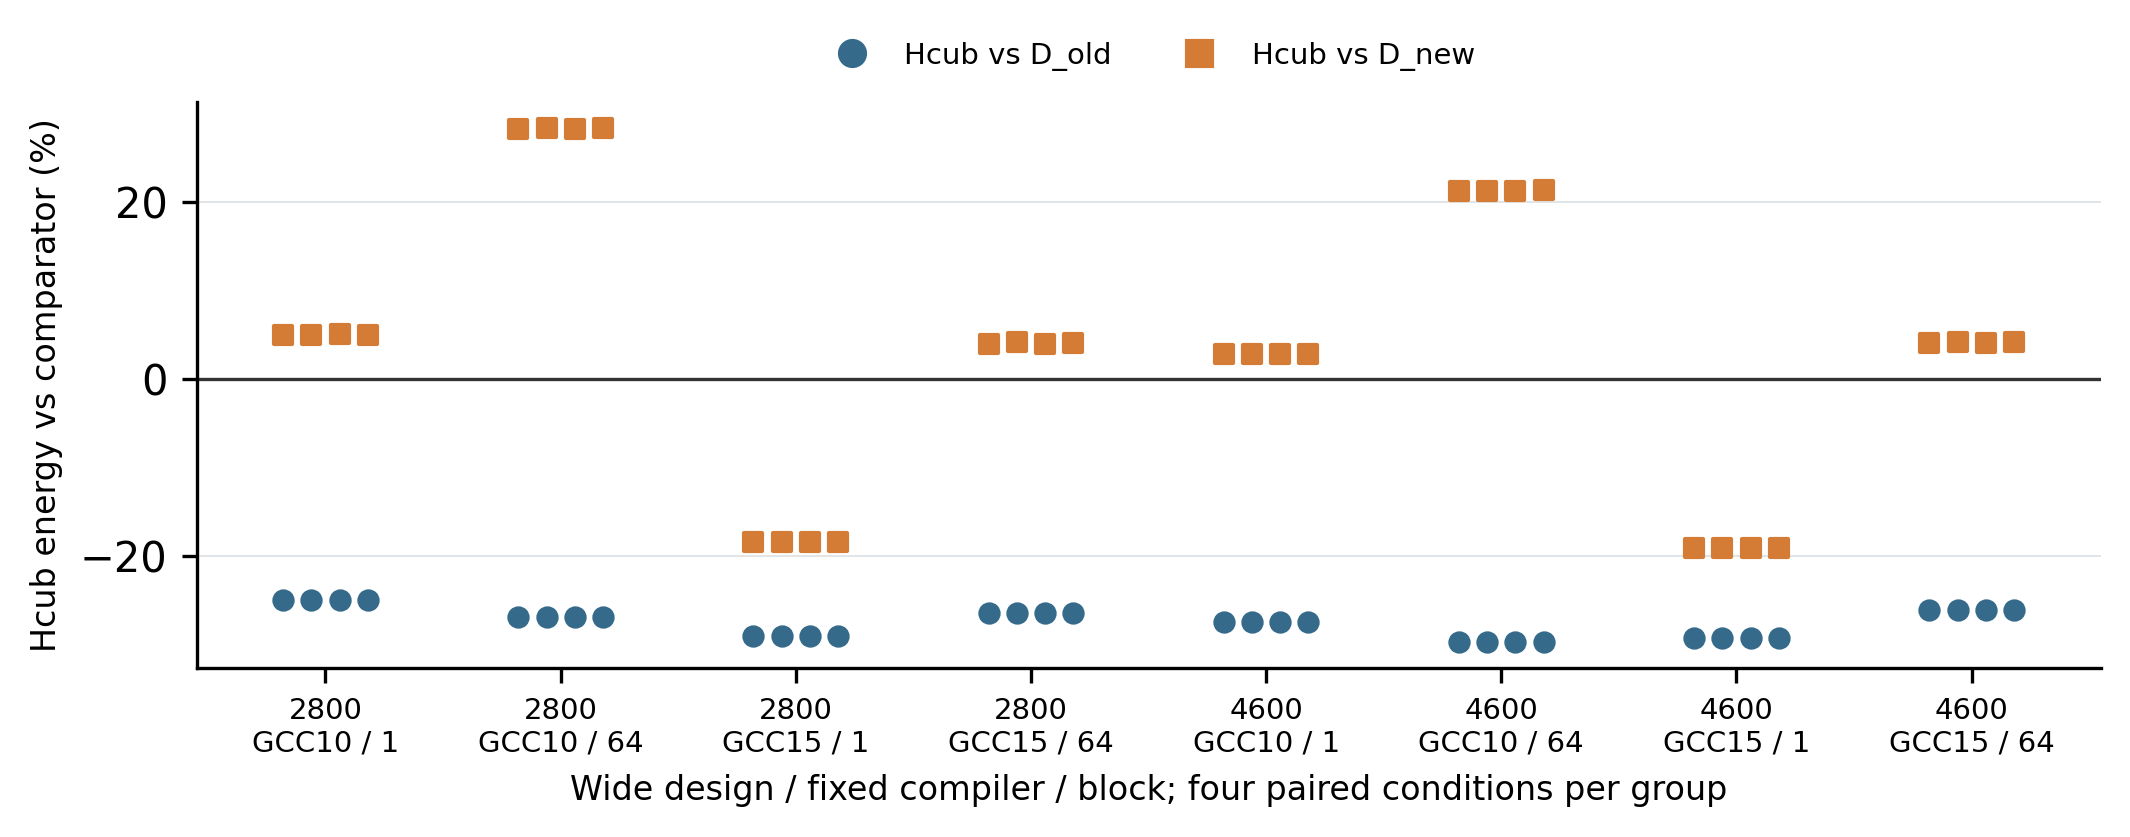
\includegraphics[width=\textwidth]{figures/panel-boundaries.png}
\caption{Every complete wide-design fixed-compiler boundary. Hcub relative to the old and strengthened nontransposed minima crosses from below to above zero in 24 of 32 cells. GCC15/block1 supplies the eight nonreversals. Within each group, points run left to right as ADC/startup, ADC/post-startup, full/startup and full/post-startup. Eight unavailable native fast-CMSIS/block64 identities leave the full panel incomplete.}\label{fig:figures-panel-boundaries.png}
\end{figure*}

\section{Discussion and limits}\label{discussion-and-limits}

\subsection{Contribution and pursuit verdict}\label{contribution-and-pursuit-verdict}

Arithmetic-fair direct correction changes two original implementation
decisions; the fresh wide-required panel supplies 24 complete fixed-cell
witnesses to the same comparator boundary. Yet incremental sharing loses
in every fresh wide cell. That adverse result matters: a nominal win
over old direct/library controls can coexist with no gain from sharing
within transposition. The compiler split, tied partitions and
unavailable native cells prevent a simple width-based selector.

The planned upgrades have distinct contribution roles. U1's controlled
framing and U4's portable evidence are supporting scholarship. U2 adds
exact artifact-specific event tradeoffs and sensitivity boundaries, with
no new analysis method. U3 supplies bounded prospective wide-design
witnesses while leaving the full panel incomplete; it does not establish
representative prevalence or beneficial sharing on fresh wide designs.

U5 passes its stronger local conjunction: reviewed preparation
disappears, GCC15 cost falls and the compiler gap contracts past zero.
This strengthens the account that callee-visible block knowledge
matters, while broader code changes prevent exclusive attribution to
rotation removal. The combined outcomes support pursuing the work as a
bounded empirical case study with auditable controls and mechanism
evidence. They establish neither a new algorithm nor field priority, an
implementation selector or publication acceptance.

\subsection{Internal and external validity}\label{internal-and-external-validity}

Arithmetic proofs, graph algebra, UBSan, finite output/state/guard
checks, binary identity and emitted-code review address different
failure modes. Output agreement alone proves neither C-language safety
nor model validity. The tested direct cuts/schedules/options are finite
controls, not an exhaustive optimization search. Their pre-cost freeze
prevents outcome-driven replacement.

The original ADC stream spans −1024 to 1023: its bound
\(1024\times72509=74249216\) limits output magnitude to 2266 without
saturation. The new full-range inputs exercise source clamps but are
still finite synthetic stimuli. Three gain-normalized arrays at one
length cannot establish application prevalence. Neither static
full-domain legality nor a post-startup segment turns those stimuli into
exhaustive performance coverage or proven steady state. The chronology
separates old development evidence from the fresh panel.

Single-cycle MUL, zero waits and frequency/prefetch settings are model
assumptions. Board current, peripheral energy and physical uncertainty
are unmeasured. Reweighting fixed events does not simulate another
configuration, which could change the events themselves. The block1
direct intervention has a satisfied \(b=1\) precondition and cannot
establish block64 behavior, other-form rankings or compiler-pass
causation.

Resources constrain adoption separately from modeled energy. Original
direct state allocation is 98/224 bytes at blocks 1/64, versus
transposed192. Its process frames and selected symbols (Appendix A)
exclude full call-chain/image costs. The new panel additionally admits
actual linked-memory and conservative stack-chain bounds. These metrics
remain distinct rather than summed as RAM.

\subsection{Evidence portability and reproduction levels}\label{evidence-portability-and-reproduction-levels}

The original 531-file raw-evidence slice includes
source/binaries/disassembly/ logs, certificates, Hcub notices, checker
code and dependency identities. A restored clean copy regenerated the
numerical report and checked 24 historical, four partial-direct and two
explanation rows, including 29 explanation hashes, with zero skips.
Explicit copied roots prevent original-workspace fallback. Those check
levels overlap in underlying binaries; they are not additional disjoint
target experiments. The extended package was exercised separately.

Table regeneration, saved-binary verification and new target execution
are distinct levels. Executable toolchain trees are excluded; rebuilding
needs separately acquired pinned GCC10/GCC15, simulator and CMSIS/Hcub
dependencies, with acquisition/identity instructions. Hash consistency
detects changed bytes, not authenticity or physical validity. No public
archive or DOI is claimed.

The upgraded package contains 7,266 manifested payload files. A fresh
relocated copy passed all seven verification commands: original
numerical regeneration, 24 historical/four partial-direct raw checks,
two explanation checks with 29 evidence hashes, exact U2 regeneration,
panel performance and correctness checks, and the intervention audit.
The panel audits admitted 280 performance identities with eight
scientifically unavailable and zero failed, and 70 correctness
identities with two expected unavailable and zero failed. The
intervention audit admitted four performance and four correctness rows.
All seven commands exited successfully, with zero integration skips and
zero target-tool executions. Scientific unavailability remains an
explicit result of the frozen panel and does not represent skipped
verification. This exercise establishes portability of the saved
evidence and regenerable analyses at the stated levels, rather than a
fresh target rebuild or physical replication.

\section{Conclusion}\label{conclusion}

Arithmetic-fair direct correction overturns two original Hcub decisions
and supplies 24/32 complete-wide prospective reversal witnesses, with
unavailable native cells keeping the full panel incomplete. Beneficial
incremental sharing does not extend to either fresh wide design:
ordinary transposition wins that contrast throughout. Saved events
expose RAM-sensitive margins, and a matched literal-one direct
specialization removes next-output preparation, lowers cost and reverses
the compiler gap. These finite results make comparator arithmetic, state
representation and visible API knowledge necessary parts of interpreting
this artifact's nominal winners. They support an auditable model case
study, without a new algorithm, physical saving or general
implementation rule.

\begin{thebibliography}{99}

\bibitem{1} L. De Coster, M. Adé, R. Lauwereins, and J. A. Peperstraete, ``Code
Generation for Compiled Bit-True Simulation of DSP Applications,'' in
\emph{Proceedings of the 11th International Symposium on System
Synthesis}, 1998, pp.~9--14.
\href{https://cecs.uci.edu/~papers/compendium94-03/papers/1998/isss98/pdffiles/1_2.pdf}{Primary
manuscript}.

\bibitem{2} A. Gačić, M. Püschel, and J. M. F. Moura, ``Fast Automatic Software
Implementations of FIR Filters,'' in \emph{Proceedings of IEEE ICASSP},
vol.~II, 2003, pp.~541--544, doi: 10.1109/ICASSP.2003.1202423.
\href{https://www.researchgate.net/publication/2589071_Fast_Automatic_Software_Implementations_of_FIR_Filters}{Author-uploaded
full text}.

\bibitem{3} P. D'Alberto, M. Püschel, and F. Franchetti, ``Performance/Energy
Optimization of DSP Transforms on the XScale Processor,'' in
\emph{HiPEAC 2007}, LNCS 4367, 2007, pp.~201--214.
\href{https://users.ece.cmu.edu/~franzf/papers/hipeac07.pdf}{Author
manuscript}.

\bibitem{4} Y. Voronenko and M. Püschel, ``Multiplierless Multiple Constant
Multiplication,'' \emph{ACM Transactions on Algorithms}, vol.~3, no. 2,
Art. 11, May 2007, doi: 10.1145/1240233.1240234.
\href{https://spiral.ece.cmu.edu/pub-spiral/pubfile/synth_28.pdf}{Author
manuscript}.

\bibitem{5} K. Nikov, K. Georgiou, Z. Chamski, K. Eder, and J. Nunez-Yanez,
``Accurate Energy Modelling on the Cortex-M0 Processor for Profiling and
Static Analysis,'' in \emph{2022 29th IEEE International Conference on
Electronics, Circuits and Systems (ICECS)}, 2022, pp.~1--4, doi:
10.1109/ICECS202256217.2022.9971086. Accessible version:
arXiv:2301.12806v1, 2023.
\href{https://arxiv.org/html/2301.12806v1}{Primary paper}.

\bibitem{6} D. Ménard and O. Sentieys, ``DSP Code Generation with Optimized Data
Word-Length Selection,'' in \emph{SCOPES 2004}, 2004, pp.~214--228, doi:
10.1007/978-3-540-30113-4\_16.
\href{https://www.researchgate.net/publication/220905057_DSP_Code_Generation_with_Optimized_Data_Word-Length_Selection}{Author-uploaded
manuscript}.

\bibitem{7} GNU Project, ``Optimize Options,'' \emph{GCC Online Documentation}.
\href{https://gcc.gnu.org/onlinedocs/gcc/Optimize-Options.html}{Official
documentation}.

\bibitem{8} SciPy developers, ``scipy.signal.minimum\_phase,'' \emph{SciPy 1.15.3
Reference}.
\href{https://docs.scipy.org/doc/scipy-1.15.3/reference/generated/scipy.signal.minimum_phase.html}{Pinned
API documentation}.

\bibitem{9} Arm, ``Finite Impulse Response (FIR) Filters,'' \emph{CMSIS-DSP
Documentation}.
\href{https://arm-software.github.io/CMSIS-DSP/main/group__FIR.html}{Official
arithmetic/storage guidance}. Current guidance supplies context; the
artifact's pinned v1.14.4 source and compiler admission govern the
actual library paths.

\bibitem{10} ACM SIGSIM-PADS 2026, ``Artifact Evaluation.''
\href{https://sigsim.acm.org/conf/pads/2026/blog/artifact-evaluation/}{Official
artifact guidance}. Used as an established practice reference, not a
binding venue rule.

\end{thebibliography}

\appendices

\section{Original principal-row resource diagnostics}\label{appendix-a.-original-principal-row-resource-diagnostics}

Cycles are estimated per requested output. Code is selected
kernel/coefficient symbols, excluding fixture and possibly helper code;
frame is the compiler's static \texttt{probe\_process} report; state is
allocated state including block capacity. These are not total image,
peak stack or SRAM high-water measurements.

\begin{table}[!t]
\centering\footnotesize
\setlength{\tabcolsep}{2pt}
\caption{Every original principal-row resource diagnostic.}\label{tab:12}
\begin{tabularx}{\columnwidth}{@{}>{\raggedright\arraybackslash}X>{\raggedright\arraybackslash}X>{\raggedright\arraybackslash}X>{\raggedright\arraybackslash}X>{\raggedright\arraybackslash}X>{\raggedright\arraybackslash}X@{}}
\toprule
Cell & Form & Cycles/out. & Code, B & State, B & Frame, B \\
\midrule
GCC10/1 & CMSIS & 1585.11 & 1494 & 112 & 8 \\
GCC10/1 & Wide direct & 1606.11 & 1736 & 98 & 440 \\
GCC10/1 & Partial direct & 1065.11 & 1036 & 98 & 72 \\
GCC10/1 & Ordinary transposed & 1106.11 & 1540 & 192 & 272 \\
GCC10/1 & Hcub & 1150.11 & 1504 & 192 & 344 \\
GCC10/64 & CMSIS & 924.32 & 1494 & 236 & 8 \\
GCC10/64 & Wide direct & 1029.33 & 1720 & 224 & 440 \\
GCC10/64 & Partial direct & 583.31 & 1196 & 224 & 72 \\
GCC10/64 & Ordinary transposed & 630.64 & 1540 & 192 & 272 \\
GCC10/64 & Hcub & 636.40 & 1504 & 192 & 344 \\
GCC15/1 & CMSIS & 1550.11 & 1450 & 112 & 8 \\
GCC15/1 & Wide direct & 1798.11 & 1872 & 98 & 608 \\
GCC15/1 & Partial direct & 1365.63 & 1372 & 98 & 240 \\
GCC15/1 & Ordinary transposed & 1100.11 & 1532 & 192 & 272 \\
GCC15/1 & Hcub & 1062.11 & 1352 & 192 & 344 \\
GCC15/64 & CMSIS & 851.98 & 1450 & 236 & 8 \\
GCC15/64 & Wide direct & 1074.65 & 1884 & 224 & 608 \\
GCC15/64 & Partial direct & 612.39 & 1312 & 224 & 232 \\
GCC15/64 & Ordinary transposed & 627.57 & 1532 & 192 & 272 \\
GCC15/64 & Hcub & 593.49 & 1352 & 192 & 344 \\
\bottomrule
\end{tabularx}
\end{table}

\section{Editable evidence map}\label{appendix-b.-editable-evidence-map}

The original manuscript/results remain preserved under
\texttt{research/fir-paper/}. Its
\href{../../fir-paper/source-manifest.json}{source manifest} records six
frozen numerical inputs. The original coefficient and timed-input SHA256
values are
\texttt{\seqsplit{63796e3e365dbdee70192acf68f16f403802d961df48ae814ffb23cca411fb70}}
and
\texttt{\seqsplit{d952c2754c9ae922243966a9c2533a848b345aa2d2d6cb5b4e68d9df1615f310}}.
The \href{../analysis/analysis.json}{saved-event analysis} retains
source digests, 12 oriented identities, exact difference vectors, cost
components, cycle and separate resource deltas, rational boundaries and
endpoint winners. The \href{../README.md}{portable-evidence
instructions}, \href{../evidence-manifest.json}{evidence manifest} and
\href{../artifact-check.json}{clean-copy report} identify the package
and verification levels.

The frozen \href{../panel-protocol.json}{panel protocol},
\href{../panel-design.json}{coefficient design},
\href{../panel-inputs.json}{inputs},
\href{../panel-certificates.json}{certificates},
\href{../vendor/graphs-manifest.json}{graph manifest} and
\href{../sources-manifest.json}{source manifest} bind the prospective
preparation. The \href{../panel-results.json}{panel identity inventory},
\href{../panel-summary.json}{exact summary} and
\href{../verification/independent-audit.json}{independent raw audit}
preserve every condition, event vector, tie, unavailable identity and
paired contrast. These panel results have passed independent scientific
review. The \href{../intervention-results.json}{intervention inventory}
binds four performance and four correctness rows to their raw artifacts.
Its measurements are admitted, and the
\href{../intervention-review.md}{independent emitted-code review}
accepts the preparation-removal ruling and stronger conjunction. The
automated measurement record retains a pending-review field distinct
from that manual ruling. The clean-copy report records the extended
package verification described in Section 8.3. The historical 12/24
filter-bank statistic belongs to its original candidate set; no revised
bank-wide result is inferred here.
\end{document}
